\chapter{Системное моделирование} \label{chap:system_modeling}

Пользуясь спроектированными ранее элементами составим общую схему приёмной
ячейки по примеру структурной схемы из технического задания (Рис.\ref{fig:SystemSch})

\begin{figure}[H]
	\centering
	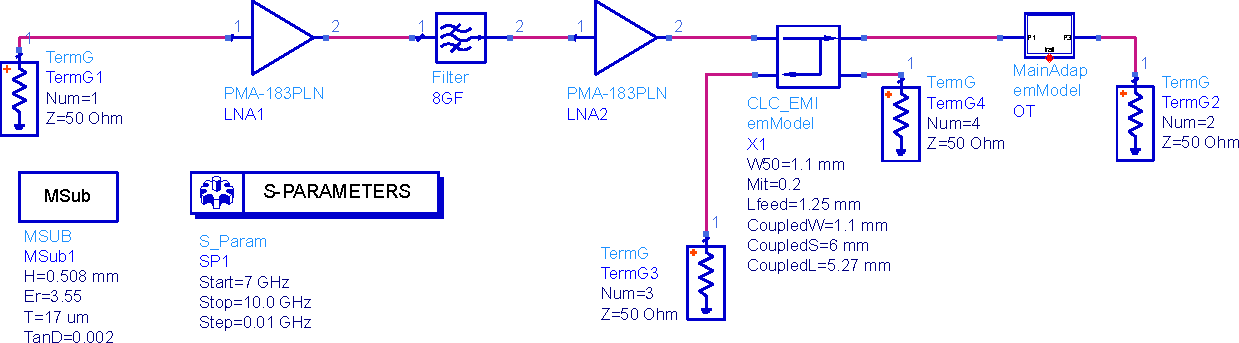
\includegraphics[width=\textwidth]{SystemSch.pdf}
	\caption{Схема проектируемой приёмной ячейки}%
	\label{fig:SystemSch}
\end{figure}

\begin{figure}[H]
	\centering
	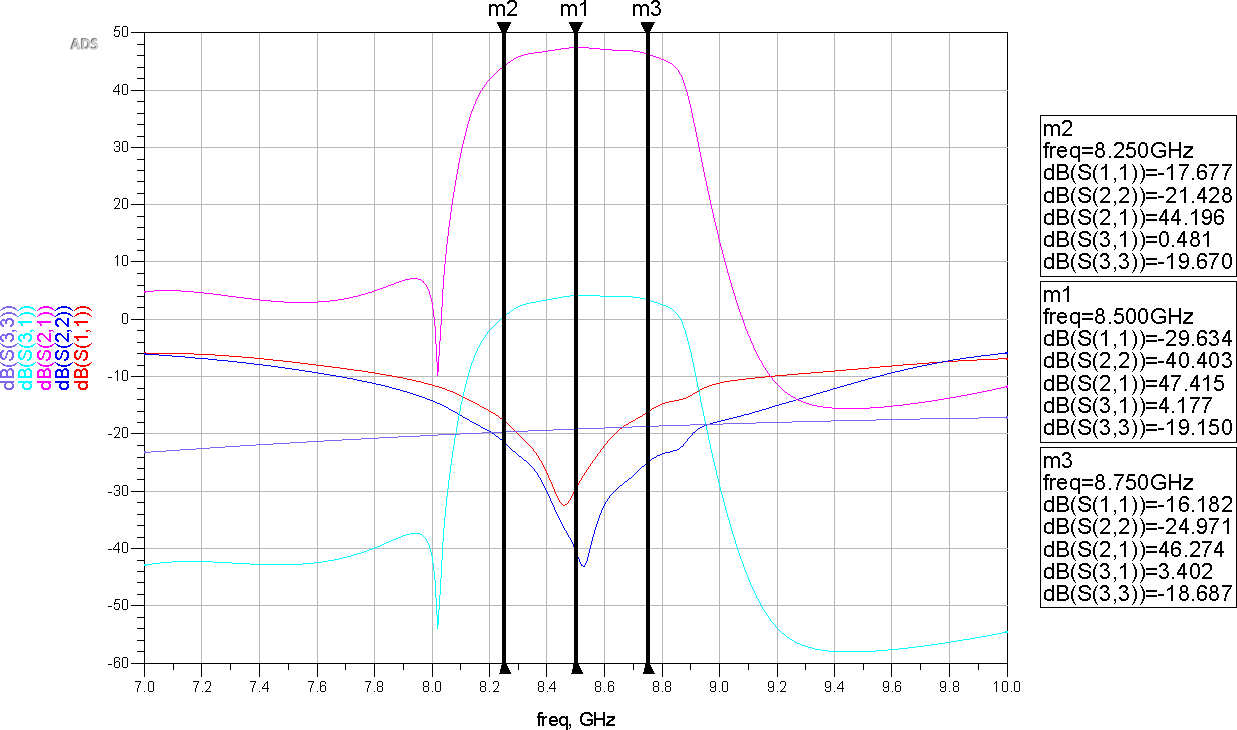
\includegraphics[width=0.9\textwidth]{SystemResponse.pdf}
	\caption{Результаты моделирования}%
	\label{fig:SystemResponse}
\end{figure}

\begin{figure}[H]
	\centering
	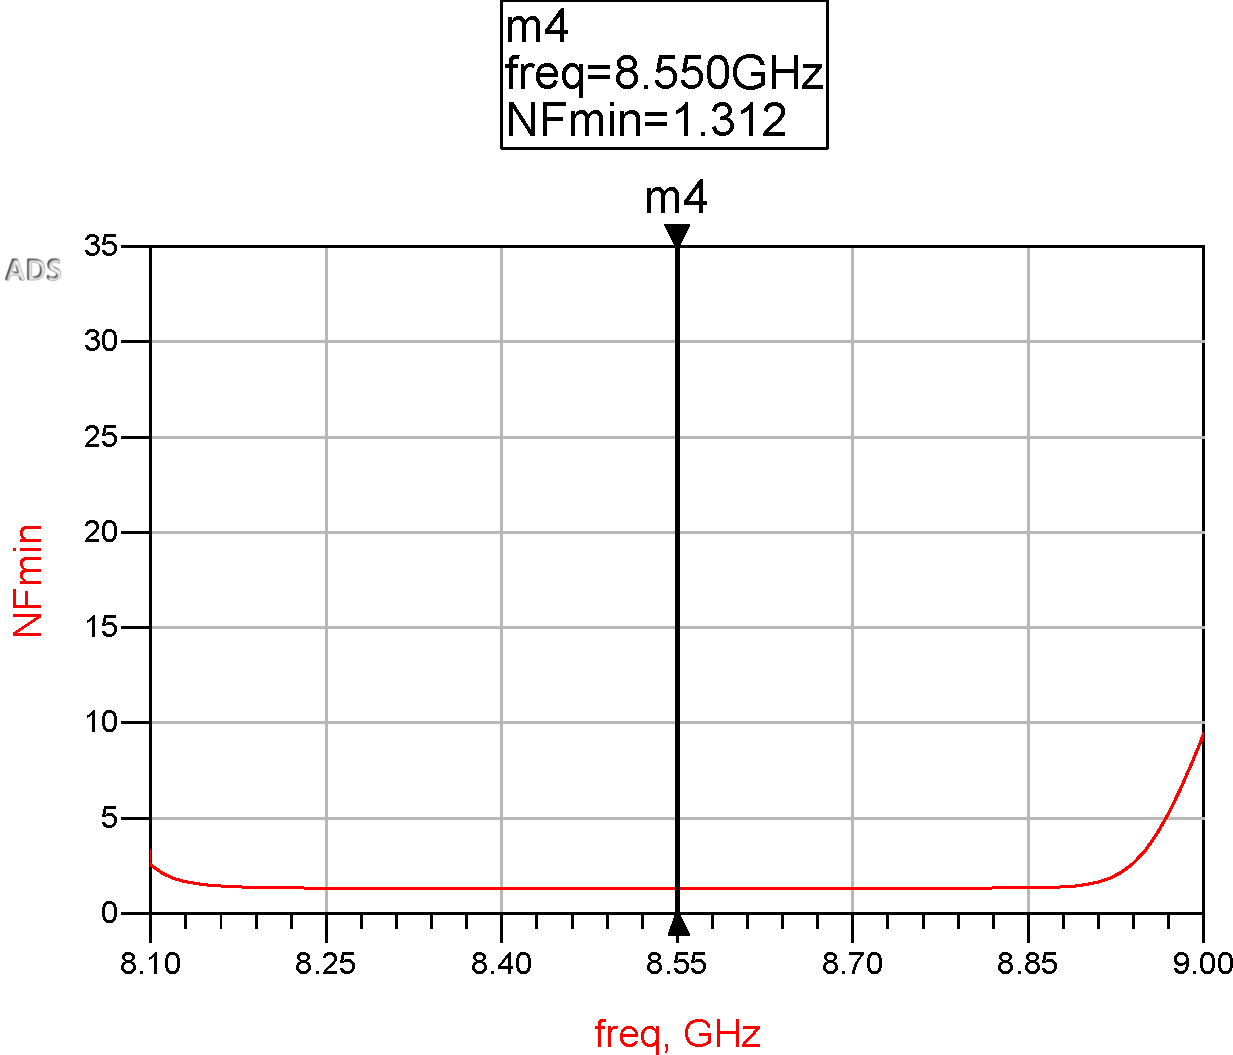
\includegraphics[width=0.8\textwidth]{SystemNF.pdf}
	\caption{Шумовые характеристики}%
	\label{fig:SystemNF}
\end{figure}

Данная модель соответствует выданному ТЗ и может быть отправлена на следующий 
этап проектирования.